%----------------------------------------------------------------------------------------
%	PACKAGES AND DOCUMENT CONFIGURATIONS
%----------------------------------------------------------------------------------------
\documentclass[11pt]{article}
\usepackage{amsmath} % Required for some math elements
\usepackage{hyperref}
\usepackage[table,xcdraw]{xcolor}
\usepackage{lipsum} 
\usepackage{cite}
\usepackage{graphicx} % Required for the inclusion of images
\usepackage{algorithmic}
\usepackage{array}
\usepackage{adjustbox}
\usepackage{bookmark}
\usepackage[margin=24mm]{geometry}


\interdisplaylinepenalty=2500 %Note that the amsmath package sets \interdisplaylinepenalty to 10000 thus preventing page breaks from occurring within multiline equations. Use: \interdisplaylinepenalty=2500 after loading amsmath to restore such page breaks as IEEEtran.cls normally does

\hypersetup{ %color attributes of citation, link, etc.
    colorlinks=orange,
    linkcolor=cyan,
    filecolor=gray,      
    urlcolor=cyan,
    citecolor=cyan,
}
%----------------------------------------------------------------------------------------
%	DOCUMENT INFORMATION
%----------------------------------------------------------------------------------------
\title{RESE412 - Project 3 Design Report \\ Remote Control Car Charge Station}
\author{Daniel Eisen}
\date{\today}

\begin{document}
\maketitle
%----------------------------------------------------------------------------------------
%	DOCUMENT CONTENT
%----------------------------------------------------------------------------------------
\section{Introduction}


\section{Environmental Conditions}
The primary and sole energy source of the charge station is solar, due to the elimination of wind due to non-functional turbine, and thus the resource examined was an solar irradiance availality as well as likely hood of external interference due to tree coverage/building occlusion and selection of array bearing and tilt.

To gather information to inform our design we utilised both NIWA solarView \cite{solarview} for historical data and on site examination to access special setup and topology.

\subsection{Solar Irradiance}
\begin{figure}[h!]
    \begin{center}
        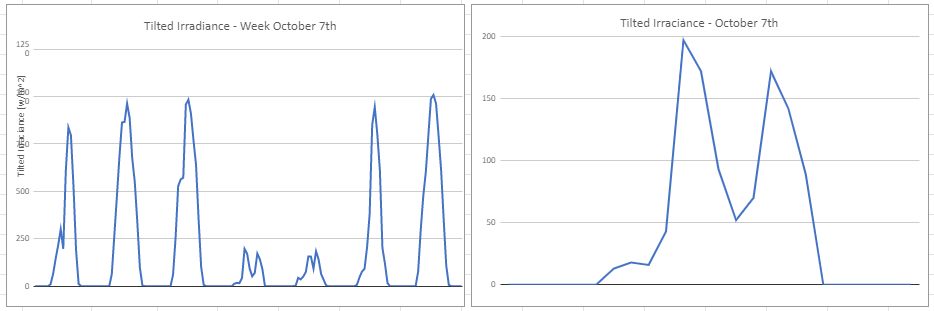
\includegraphics[width=0.5\textwidth]{inc/irr.png}
        \caption{Solar View tilted irradiance}
        \label{fig:solarview}
    \end{center}
\end{figure}

The historical data of track location, shows that on the day (October $7^{th}$) there is an expectation of significantly less nominal solar energy available. As shown \ref{fig:solarview} above the data expects a max of $200 W{\cdot}m^{-2}$ with significant midday dips. From this we can infer the very real possiblty of heavy/intermittent cloud cover.

\begin{table}[h!]
    \begin{center}
        \begin{tabular}{|l|l|}
            \hline
            \multicolumn{2}{|c|}{\textbf{Average Irr race period 11:00 - 14:00}} \\ \hline
            \textit{Oct 7th}                   & \textit{Week}                   \\ \hline
            96.75                              & 612.61                     \\ \hline
        \end{tabular}
    \end{center}
\end{table}

To prevent drastically oversizing the final design and to ensure optimising for total costing of the system, we examined the average irradiance over the race time of both the week as a whole and of the day itself (see above). From this we proceeded forth with expectation that the panels may be operating at half their possible maximum output. This directly informed the amount of panels we chose in order to supply our energy requirements, especially due to possible large fluctuation erring on a robust rather than exactly matched system.

\subsection{Topology}

\begin{center}
    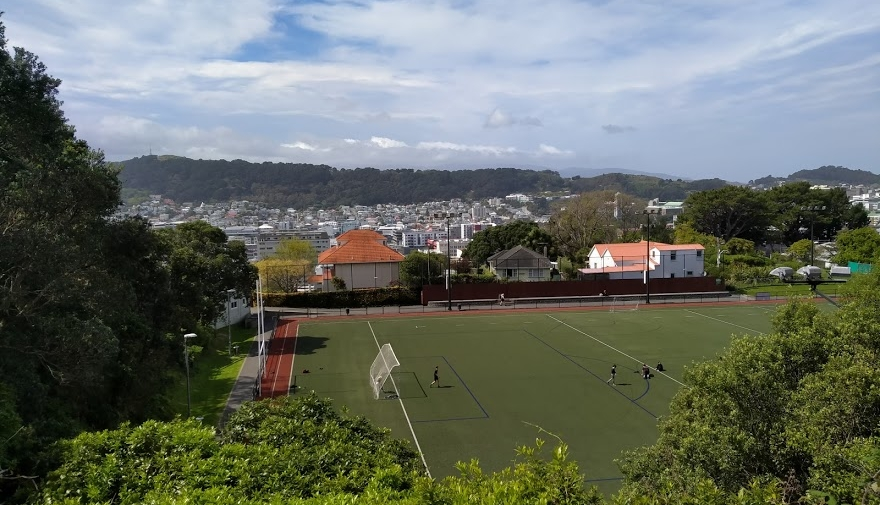
\includegraphics[width=0.5\textwidth]{inc/IMG20201006120746.jpg}
\end{center}

By visiting the site during the time on the week off the race, we were able to make an inspection of effects of shadows from building and trees. Seen above, the tree coverage of the northern tree line does not infringe on the section of field intended for solar collection, nor do any building. Therefore we can directly use the NIWA data under assumtion that the only occlusion of direct sun we would experience would be cloud coverage.

\section{Race/Track Conditions}
\begin{figure}
    
\end{figure}
\begin{center}
    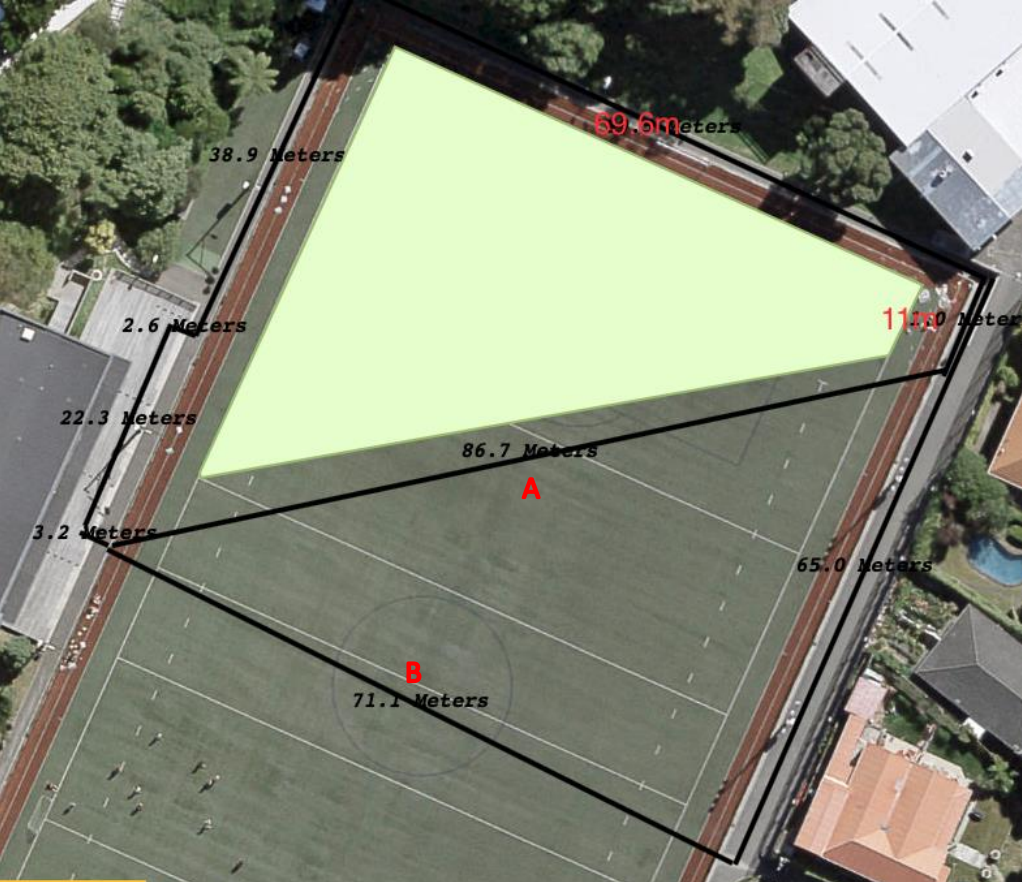
\includegraphics[width=0.5\textwidth]{inc/tracks.png}
    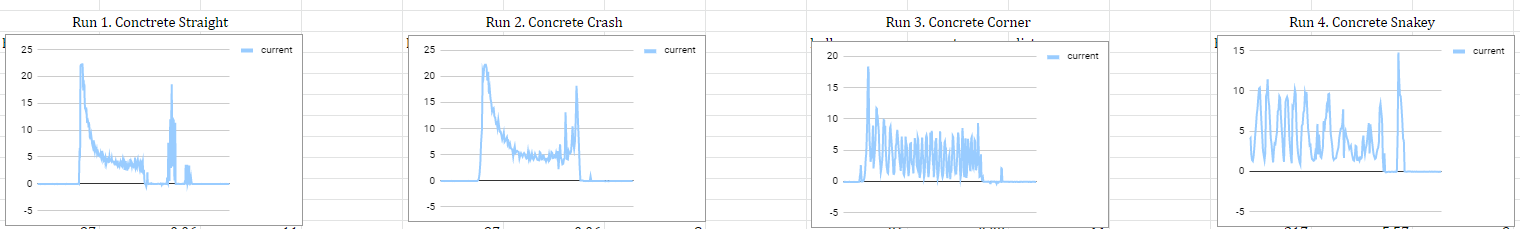
\includegraphics[width=\textwidth]{inc/contrete_behaviour.png}
    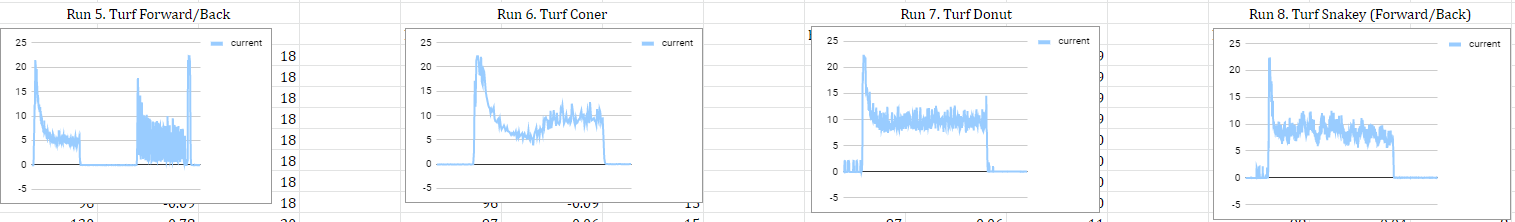
\includegraphics[width=\textwidth]{inc/turf_behaviour.png}
\end{center}
\section{Component Testing}
\subsection{Battery Capacity and Charge Time}
\subsection{Motors}

\begin{figure}[h!]
    \begin{center}
        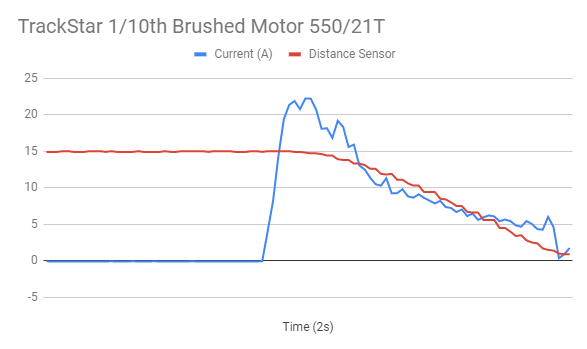
\includegraphics[width=0.3\textwidth]{inc/large_motor.png}
        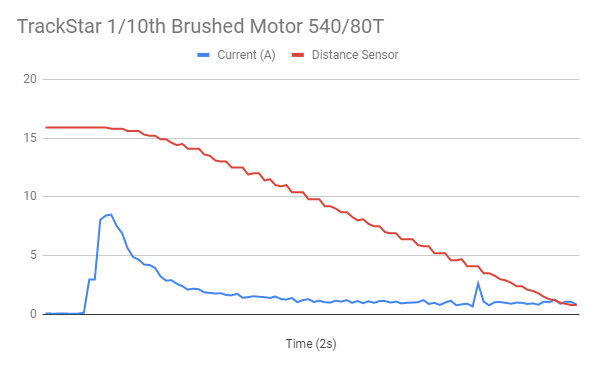
\includegraphics[width=0.3\textwidth]{inc/slow_motor.png}
        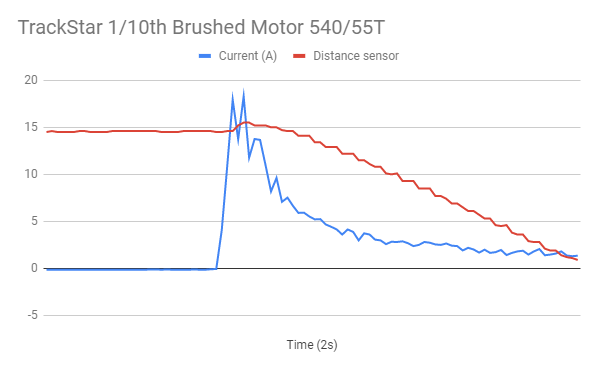
\includegraphics[width=0.3\textwidth]{inc/small_motor.png}
    \end{center}
\end{figure}

\section{System Design}
\subsection{Charge Station}

\begin{center}
    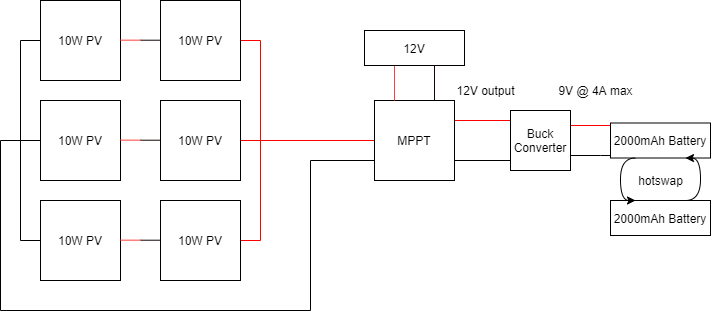
\includegraphics[width=0.5\textwidth]{inc/panels.png}
\end{center}

\subsection{Car}

\begin{figure}[h!]
    \begin{center}
        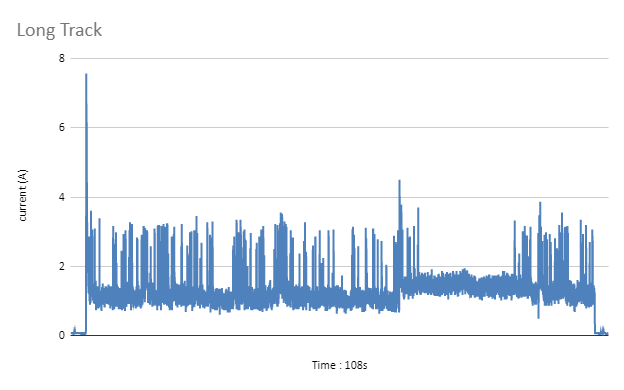
\includegraphics[width=0.3\textwidth]{inc/long_lap.png}
        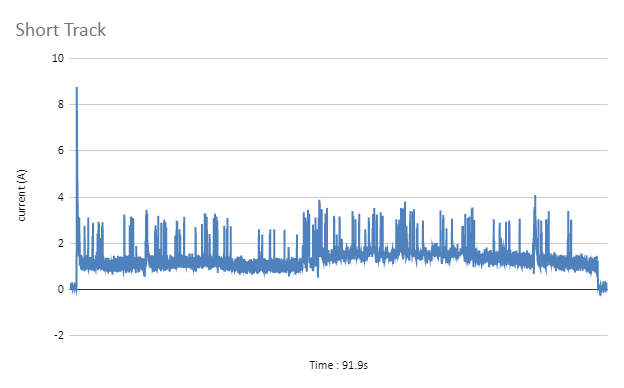
\includegraphics[width=0.3\textwidth]{inc/short_lap.png}
    \end{center}
\end{figure}

\section{Risk Analysis}

\section{Budget}

\begin{table}[h!]
    \begin{center}        
    \begin{tabular}{|l|l|}
    \hline
    \multicolumn{2}{|c|}{\textbf{Team ECO Budget}}            \\ \hline
    6 x 12V 10W Polycrystalline solar panel & 285.42 \\ \hline
    buck                                    & 12.39  \\ \hline
    MPPT + 12V bat                          & 86.85  \\ \hline
    2 x NiMH battery 2000mAh                & 154.44 \\ \hline
    TrackStar 1/10th Brushed Motor 540/80T  & 14.04  \\ \hline
    \textbf{total}                          & \textbf{553.14} \\ \hline
    \end{tabular}
    \end{center}
    \end{table}
\section{Conclusion}

\bibliography{ref}
\bibliographystyle{IEEEtran}
\end{document}
